\documentclass[../dissertation.tex]{subfiles}
\begin{document}

\chapter{Research}
\label{sec:research}

\section{Background}
\label{sec:background}

Initial research was completed over a three month period and covered network visualisation, specifically massive network visualisation, and additionally looked into software that existed which visualised networks. The dearth of previous research confirmed that this is an area that was worth exploring further. This meant that exploration had to be done from scratch as there was no previous studies to build upon. However, this proved advantageous as the wealth of information gained during this period informed future decisions throughout the project.

In regards to the visualisation of massive networks, some important techniques learnt were:

\subsection{Node Bundling}
\label{sec:node_bundling}

Node Bundling is using algorithms to decide (with or without some form of user input) which nodes are similar to each other, and upon establishing this relationship, grouping them into a single node, generally visually different in some way (often by size or colour). It ``creates a less complicated visualization without losing connectivity information by automatically abstracting small [...] subgraphs'' \cite{six2003effective}. This allows for hundreds or thousands of nodes to be grouped into a single node in order to require less memory, processing power, bandwidth and screen space on the users machine. A way to further improve the visualisation is to show how the nodes being bundled connected with themselves, for example if they are heavily connected, all connected to just a few nodes, or if they are in a ring formation. Figure \ref{fig:bundling} and \ref{fig:deletion} demonstrate both node and edge bundling.

\subsubsection{Node Pruning}
\label{sec:node-pruning}

An example of a node bundling algorithm is `Node Pruning'. This is a technique that takes each node in a network with only one edge and deletes it from the network. This can often reduce the number of nodes in a network by a significant amount, while retaining its overall shape. The algorithm is mentioned in literature as a step to creating a bundled network but is not named \cite{brandes2003experiments}. Hence, for the purpose of this dissertation, it was named `Node Pruning'. More information about Node Pruning can be found in Section \ref{sec:impl-node-prun}.

\subsubsection{Node Bundling based on cliques}
\label{sec:node-bundling-cliques}

Another example of node bundling is an algorithm based on cliques. This involves analysing each node and deciding which are closest to cliques, with a clique being defined as every node is adjacent to every other \cite{roberts1971characterization}. The result of this is highly interconnected groups of nodes becoming bundled into one node. More information about Node Bundling based on cliques can be found in Section \ref{sec:impl-node-clique}.

\subsection{Edge bundling}
\label{sec:edge_bundling}

This is similar to node bundling but applied to edges. It ``trade[s] clutter for overdraw by routing related edges along similar paths'' \cite{hurter2012graph}, and ``can be seen as sharpening the edge spatial density, by making it high along bundles and low elsewhere'' \cite{hurter2012graph}. Overdraw is defined as making edges longer than necessary \cite{gansner2011multilevel}. If node bundling is done, then this process will have less of an impact, as all of the edges will already be bundled together assuming the node bundling algorithms were optimal. This would imply all interconnected nodes have been bundled so there is only one edge traversing between subgroups as opposed to many. Like node bundling, it is often shown through the change of the size of the edge or the colour. See Figure \ref{fig:bundling} and Figure \ref{fig:deletion} for two examples of a combination of node and edge bundling.
\begin{figure}[htb]
    \centering
    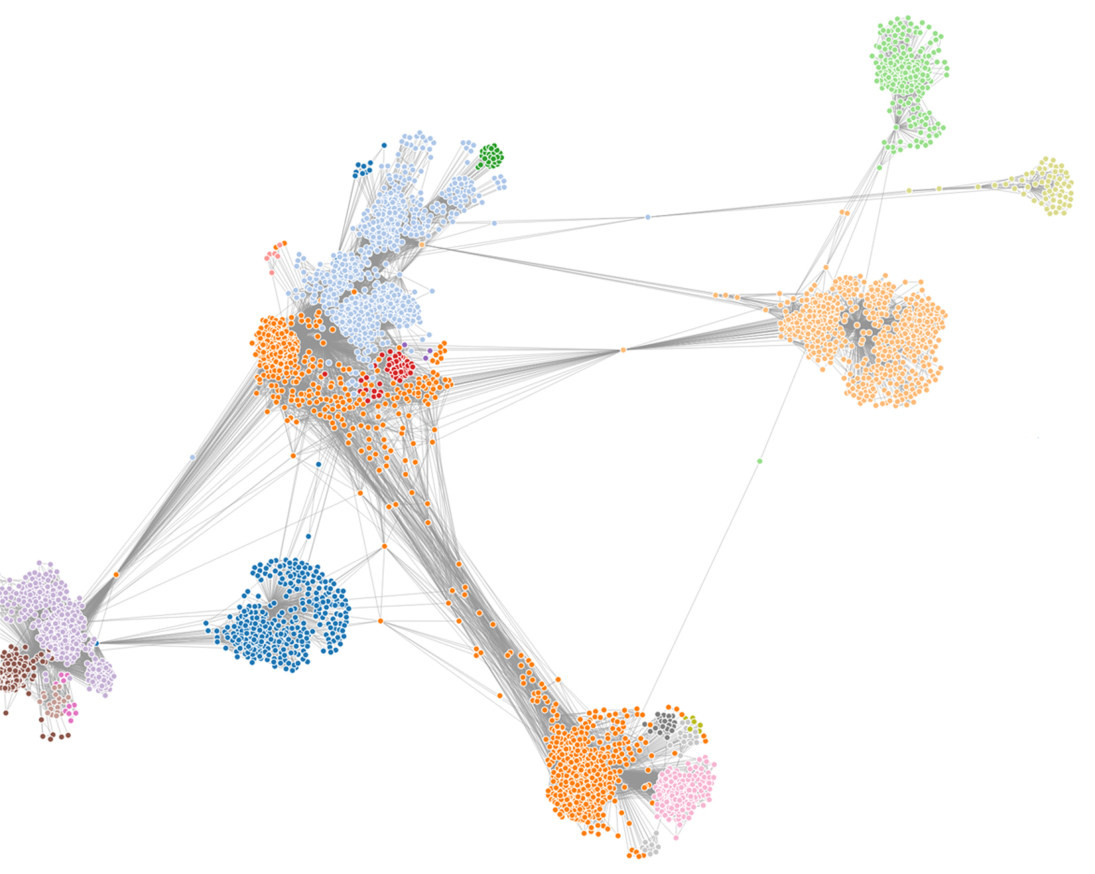
\includegraphics[width=12cm]{4/bundling1}
    \\$\downarrow$\\
    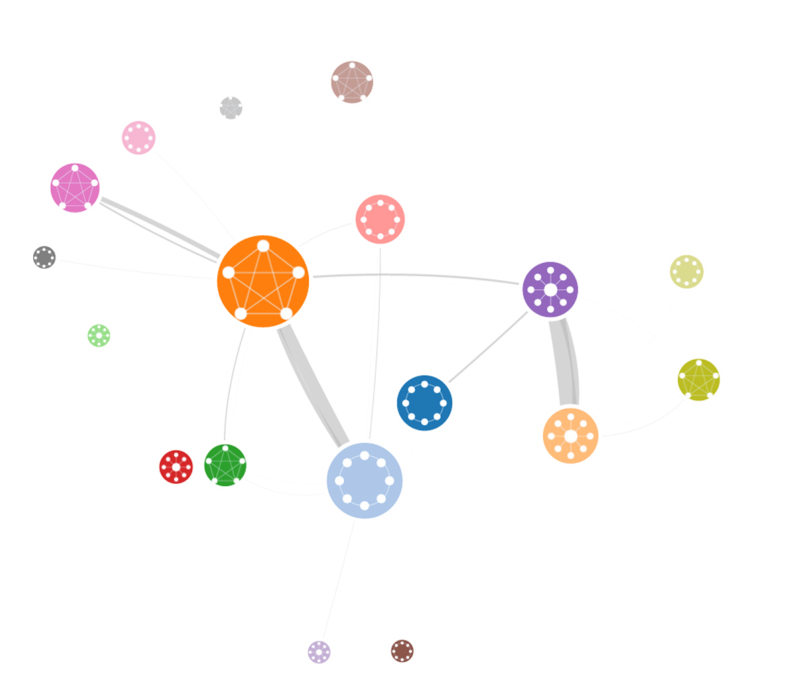
\includegraphics[width=12cm]{4/bundling2}
    \caption{This demonstrates both node and edge bundling, where thickness of edge displays how many edges there are, and size of node indicates number of nodes group. Additionally, each node displays how nodes within it were connected together. This particular example displays a comparison between a common network visualisation and a ModulGraph-based network visualisation. \cite{li2015modulgraph}}
    \label{fig:bundling}
\end{figure}

\begin{figure}[htb]
    \centering
    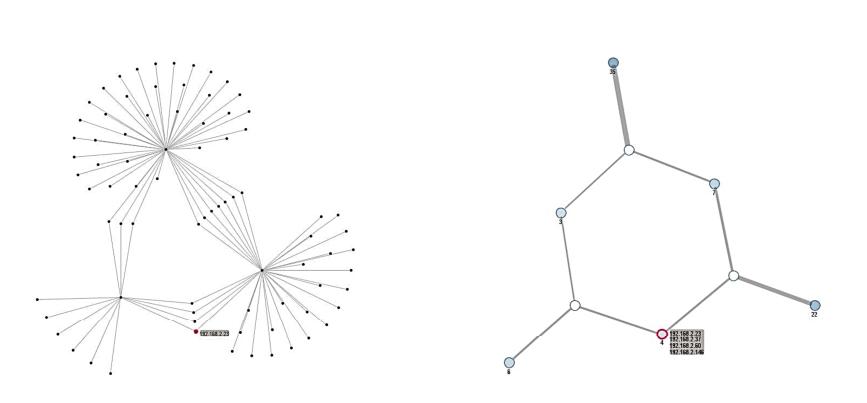
\includegraphics[width=15cm]{4/deletion}
    \caption{This figure shows how the bundling of many nodes mean that, although information is lost, the visualisation can become more clear as a result of the operation. \cite{hu2015visualizing}}
    \label{fig:deletion}
\end{figure}

\subsection{Local Edge Lens}

This involves rendering all or part of the network, and upon focusing on a section of the network, that part is zoomed in or clarified as if through a lens and that part of the network is zoomed in, becoming more clear. This can be through hiding edges that are not connected to the highlighted nodes, or rendering more information that was not shown before in order to save computational power. ``By doing so, the cluttering of edges is removed for a local focus region defined by the position and scope of the lens'' \cite{tominski2006fisheye}. See Figure \ref{fig:local} for an example of system using a local edge lens.
\begin{figure}[htb]
    \centering
    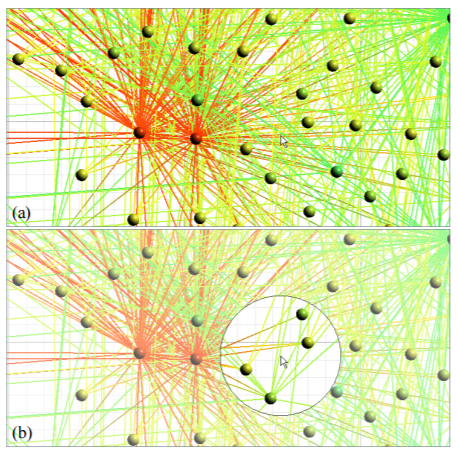
\includegraphics[width=8cm]{4/local}
    \caption{If a network is cluttered (a), then it can be hard to get useful information from it. A local edge lens (b) lets users easily identify which edges are connected to which nodes. \cite{tominski2006fisheye}}
    \label{fig:local}
\end{figure}

\section{Current Network Visualisation Software}

In addition to finding out techniques used by software for large network visualisation, a list was created of all software that was mentioned in papers or found during research that was related to large network visualisation. Quite often, the software mentioned had been hand-made for that project and was not feature complete, or the software could only be used for a price, but the below list contains the names of software that had been complimented as high quality network visualisation software - and was consequently further researched in Chapter \ref{sec:systematic-review}.
\begin{itemize}
    \item GUESS \cite{guess}
    \item SNAP \cite{snap}
    \item Gephi \cite{gephi}
    \item GraphViz \cite{graphviz}
    \item Tulip \cite{tulip}
    \item D3.js \cite{d3}
    \item Vis.js \cite{vis}
\end{itemize}

\end{document}